% !TeX spellcheck = en_GB
\documentclass[a4paper,11pt,notitlepage]{article}
\include{structure}
\hyphenation{Some-long-word}
\usepackage{amsmath}
\usepackage{fullpage}
\usepackage{graphicx}
\usepackage[english]{babel}
\usepackage{float}
\usepackage{listings}
\usepackage{color,soul}
\usepackage{pdflscape}
\usepackage[hyphenbreaks]{breakurl}
\usepackage[hyphens]{url}
\usepackage[margin=1cm]{caption}
\usepackage{subcaption}

% Title Page
\title{Laughter Detection using Neural Networks}
\author{John Scolaro\\
	Supervisor: Scott Heath\\
	Janet Wiles}

\begin{document}
%\maketitle
\thispagestyle{empty}
\begin{center}
	\begin{minipage}{0.75\linewidth}
		\centering
		%University logo
		
\includegraphics[scale=0.25]{figs/logo.jpg}
		\par
		\vspace{3cm}
		%Thesis title
		{\uppercase{laughter detector\par}}
		\vspace{3cm}
		%Author's name
		{\Large Author: John Scolaro\par}
		{\Large Supervisors: Scott Heath\\Janet Wiles\par}
		\vspace{3cm}
		%Degree
		{\Large Thesis Report\par}
		\vspace{3cm}
		%Date
		{\Large October 2016}
	\end{minipage}
\end{center}

\addcontentsline{toc}{section}{Title Page}

\clearpage

\addcontentsline{toc}{section}{Abstract}

\null\vspace{\fill}
\begin{abstract}
	This thesis proposes a new way of detecting laughter using neural networks to determine whether audio contains laughter, on a frame-by-frame level, rather than comparing large segments of audio for laughter. Several different methods are tried and tested, with the results presented here, with a simple feed forward neural network achieving the greatest accuracy, when trained on sequences of MFCC's from audio.
\end{abstract}
\vspace{\fill}

\clearpage

\addcontentsline{toc}{section}{Table of Contents}
\renewcommand*\contentsname{Table of Contents}

\tableofcontents

\clearpage

\section{Introduction}

% Basically a quick introduction skimming over all the topics covered in the whole report.
	% What I'm doing
	% Why it's a neat idea
	% What there already is
	% How I'm improving it
	% What the results were super briefly



\subsection{Motivation}

% Why I am trying to do it

Laughter classification is potentially useful for a large number of reasons.

Nobody else has done it this particular way before.

Extracting information from audio has many uses, including speech recognition and song detection, which many people use every day. In audio recordings of human speech, more information is present than just
the spoken words. Humans can glean information from the speaker, from the speed at which they talk, the tone and volume used,\cite{dellaert1996recognizing} or perhaps the amount of fillers, `umming' and `ahhhing', between sentences.\cite{brennan1995feeling} The mood of the speaker gives further information about what their words mean, and how they feel. Being able to detect these various audio cues allows for better interpretation of the sentiments underlying
human speech. Examples of systems which utilise these additional audio features include anger detection, which could be implemented in call centres to route frustrated callers directly to humans operators,\cite{yacoub2003recognition} or the detection of applause, which can be used to segment video and summarize large events.\cite{cai2003highlight} One of the most prominent non-verbal features of human speech is laughter as it gives information about the
mood of the laugher and can be associated with several emotions.

\subsection{Aim}

% What it is what I'm trying to do

Design an algorithm to detect laughter as best it can.

From this, can we learn anything about the structure of laughter from what our algorithm decides on?

Can we learn anything interesting about sequence detection with neural networks?

\section{Background}

% An in depth look into the state of the field of study so far

\section{Methodology}

% How I've gone about my work. So this is the major heading talking about what I've done to attempt to detect laughter.
% I am unsure about whether to actually put any writing about anything in this section, or just put it all into the subsections.

\subsection{Dataset}

% Starting with all my working into the dataset.
	% Talk about the audio of the dataset first.
		% How it was recorded
		% When
		% What it was for
		% The type and quality of audio
		% General statistics about the laughter.
		% Compare my dataset to other datasets and talk about the differences.
	% Preprocessing of the dataset. Removing noise. Normalizing volume roughly.
	% Talk about classification of laughter
		% My classification.
		% Compared to other peoples classification and maybe error analysis.

The dataset used for this project was a collection of recorded spontaneous speech from the Australian National Corpus. A total of eighty-one different audio clips was used, for a total audio length of fifteen hours and twenty-six minutes. These audio snippets contained conversations from students in the school yard, interview type scenarios, casual around-the-house conversation, and a variety of people in different scenarios. A majority of the recordings were taken over twenty years ago on cassette tape, and have been since converted to digital format. Conversations most frequently occur between two or sometimes three people, with the occasional recording containing more. This is important to note, as this thesis details the detection of laughter by one person, and not the detection of laughter of many people at once, as is done in other papers. [INSERT REFERENCE HERE.]\\
\\
This corpus is smaller than the datasets used in other studies, which have used hundreds of hours of audio from recorded meetings, or telephone calls. It is well known that machine learning techniques improve where there is more data, and with only fifteen hours of audio, our results will be limited. The laughter in the audio used in this study is very diverse, with many different types of laughs. There are long belly laughs from old friends, and very short polite laughs from a child addressing their parents. There are laughs from people with thick accents, and laughs emitted which trying to talk. The diversity of the dataset used is an advantage, as any patterns learnt should be to the nature of laughter 'in-general' and not overgeneralise to a specific type of laughter, or the laughter of one person.\\
\\
All audio files are purely recordings of human speech, and do not contain noises from other sources. Other laughter classifiers [INSERT REFERENCE HERE] have trained systems to detect laughter by using a myriad of different sounds to train it. (Insert examples here when you find the reference) Detecting the difference between laughter and human speech will be more difficult, but potentially more useful as laughter is often interwoven between snippets of human speech, and not between the sounds of trains, popping bubbles, and waterfalls.

\subsubsection{Classification}

Prior to this study, the audio from the Australian National Corpus had never been used for laughter detection, and the data labels didn't exist. Past research into laughter detection used the laughter labels that meeting transcribers had attached to the transcriptions of meetings. [INSERT REFERENCE HERE] and researchers had fiddled with portions of the data themselves because they found the data labels inaccurate. [FIND REFERENCE HERE AND MAYBE QUOTE]. However, with hundreds of hours of audio, sifting through it all manually to select the laughter would be infeasible. In this study, the audio was listened to, and the laughter segments were manually selected down to the millisecond.\\
\\
The method used to classify the laughter, was to use ELAN [REFERENCE], an audio-visual transcription software, to select the sections of audio which contain laughter. ELAN outputs this data in an XML format, which is parsed into a list of times when laughter starts, and then subsequently stops. These lists of start and stop times are used when creating the dataset, and the label (in one-hot encoded form) is appended to the vector of audio features.\\
\\ 
\begin{table}[]
\centering
\begin{tabular}{|l|l|}
\hline
Total Laugh Count                     & 1456           \\ \hline
Total Length of Laughter              & 1480.1 seconds \\ \hline
Longest Laugh                         & 6.32 seconds   \\ \hline
Average Laugh Length                  & 1.01 seconds   \\ \hline
Audio File with Least Laughs Contains & 0 laughs       \\ \hline
Audio File with Most Laughs Contains  & 102 laughs     \\ \hline
\end{tabular}
\caption{A table containing statistics of the laughter classified in the complete dataset.}
\label{laughter_stats_table}
\end{table}
\begin{figure}[H]
	\centering
	\vspace{0.5cm}
	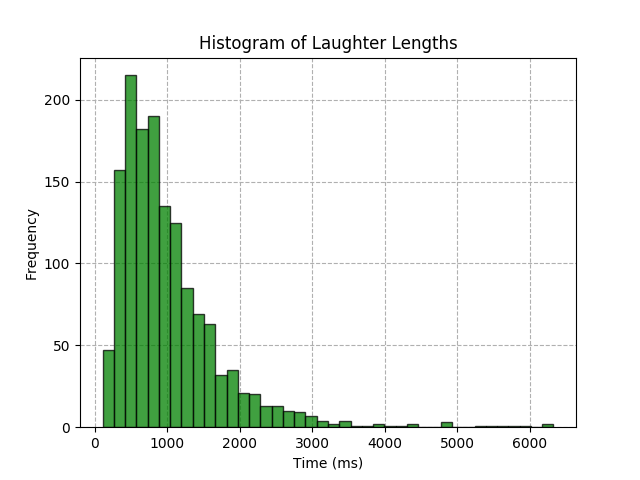
\includegraphics[scale = 0.8]{figs/laughter_length_histogram.png}
	\caption{A histogram of the laughter segment lengths.}
	\label{laughter_length_histogram}
\end{figure}
Laughter in speech is a hard audio signal to classify. It often does not have a definite start or end point. Commonly an individual laugh will be preceded by a sharp inhalation, and/or followed by a brief `ahh' sound, and every laugh is different. Some might be very quiet snickers, snorts, or just fast exhalations. What do we empirically classify as `laughter'? Rather than define `laughter' as a specific type of laughter, potentially an easily distinguishable laughter like a belly-laugh, which would make the job of classification much easier, the data was classified as what the author `felt' was laughter. In order to train a model to predict laughter as accurately as a human, it needs a human-like classification. This makes this section particularly tough to write as scientists don't enjoy saying: ``This particular section of audio `felt' like laughter'', but would rather employ some quantitative analysis to say: ''This audio is definitely laughter because...''. When it comes to machine learning with audio, we want to give the model something a human thinks is correct, and let the machine find the complex mathematical relationships which separate laughter from non-laughter.\\
\\
Nevertheless, when classifying laughter, what one person `feels' is laughter, may not be identical to the observations of another person, and this is something worth investigating. In an effort to investigate differences in laughter classification between different people, two people were taught how to classify laughter using ELAN, and given a 45 minute audio clip to classify.\\
\\
In this 45 minute clip, one classifier found 87 laughter instances, and the other found 61. The actual classifications were very similar however. The main differences are that one classifier often split longer laughter segments up into multiple pieces, and included segments of laughter interwoven with speech. Example plots of the difference classifications are shown in Figure \ref{laughter_classification_differences_1} and Figure \ref{laughter_classification_differences_2}. With more classifiers, the jerky transition between laughter and non-laughter will be smoothed. Even without more classifiers, a linear interpolation method could be employed to further smooth this transition.
\begin{figure}[H]
	\centering
	\vspace{0.5cm}
	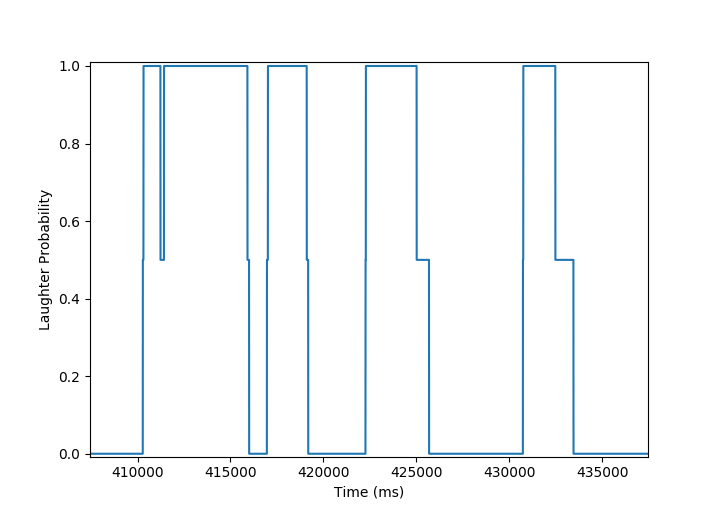
\includegraphics[scale = 0.75]{figs/differences_1.png}
	\caption{The differences in laughter classification between two different humans. Here, we see the differences in classification clearly. One classifier appears to think that laughter lasts approximately a whole second longer for the second two laughter instances, while one classifier separates the first laughter instance into two separate pieces.}
	\label{laughter_classification_differences_1}
\end{figure}
\begin{figure}[H]
	\centering
	\vspace{0.5cm}
	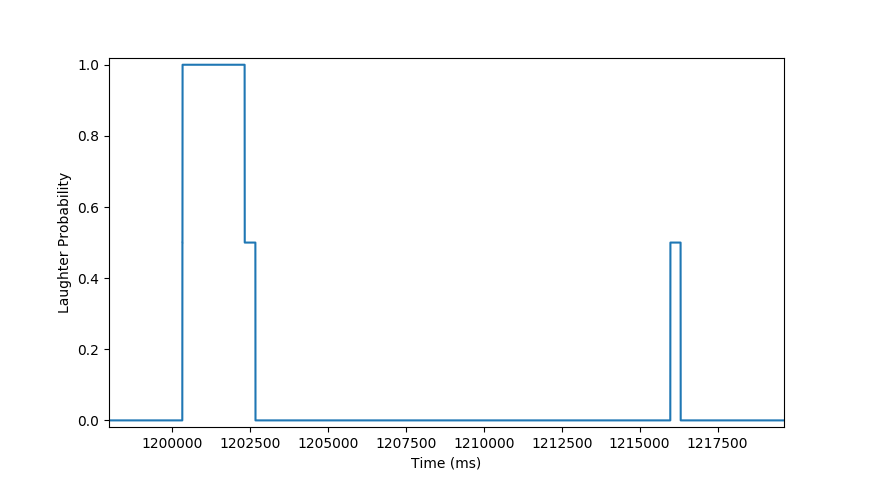
\includegraphics[scale = 0.7]{figs/differences_2.png}
	\caption{In this example, while both classifiers agree that the first laughter instance exists, only one classifier managed to find a second laughter segment.}
	\label{laughter_classification_differences_2}
\end{figure}
The entire dataset used for training the model in this report was only classified by one person, despite the promising results and improvements enabled by multiple classifications. This was due to time constraints, and the inability to convince people to listen and classify 15 hours of speech for no apparent reward. An ideal dataset should have many classifiers, and the classification used for training could be the average of all the individual classifications. This way, a section of audio which only 50\% of people think is laughter, will only be labelled as 50\% laughter, and the sections of audio at the beginning and end of laughter segments will smoothly transition from non-laughter to laughter and back, rather than an abrupt jump.

\subsection{Preprocessing}

% Noise removal and rough volume normalisation.
% mfcc extraction.
% The per-file normalisation of MFCC values.
% The data storage method for speed and size.

\subsection{Initial Analysis}

% This is performing PCA and t-SNE on the origional data and features.
	% Show that the data doesn't really appear to be especially seperable.

\subsection{TensorFlow}

% What tensorflow is, and why I chose to use it over something like MATLAB. Maybe also talk about my MATLAB results too.

\subsubsection{Input Pipeline}

% Talk about the many different input pipelines I've tried but mainly:
	% The frame by frame batches
	% The sequences of frames batches.

\subsubsection{Models}

% Talk about all the various TensorFlow models I attempted to use.
	% mlp
	% sequence mlp
	% ltsm
% Talk about additional features of the networks
	% Dropout
	% Batch normalisation
	% Shuffling
	% Activiation Function
		% Relu clipping


\subsubsection{Cost Function}

% Talk about the cost function I used. Maybe put this in the previous section or something.

\subsubsection{Initialization}

% Talk about initialization of the network.
	% Xavier Initialisation

\subsubsection{Hyper parameters}

% Show results of big tests of many different networks to find best hyper params.

\subsubsection{Training}

% Talk about my training methods and how I split data and train on it.
% Not so much because it's interesting or unique, but to show I did it correctly.

\subsubsection{Model Evaluation Metrics}

% Talk about accuracy and sensitivity and specificity.
	% Talk about all the different metrics and how I should use these to actually measure 'goodness' of the system
% Also talk about the creation of the pictures I do of the network every time I finish training.
	% The ROC curve
	% The audio probability graphs
	% The Confusion matrixes.

\section{Results}

% Talk about the metrics of the best network I made.

\section{Discussion}

% Maybe the in depth results will take place in this section, and not above.
% Talk about funky things that my networks have picked up. All the weird things.
% Different features of the audio my system is picking up.

\subsection{Improvements and Future Study}

% Talk about the myriad of features I'm sure I will have wished I could get around to, and would love to see the results of, but didn't quite have enough time to do.
% If someone else were to do this thesis, the things I would have liked them to do are:
	% Different types of laughs: genuine vs polite

\section{Conclusion}

% Conclude. Another brief summary of everything I have done, and close.

\bibliography{report}
\bibliographystyle{IEEEtran}

\end{document}
